%% LyX 2.4.0~beta5 created this file.  For more info, see https://www.lyx.org/.
%% Do not edit unless you really know what you are doing.
\documentclass[10pt]{article}
\usepackage[T1]{fontenc}
\usepackage[utf8]{inputenc}
\usepackage{geometry}
\geometry{tmargin=1in,bmargin=1in,lmargin=1in,rmargin=1in}
\usepackage{mathtools}
\usepackage{enumitem}
\usepackage{amsmath}
\usepackage{amsthm}
\usepackage{amssymb}
\usepackage{graphicx}
\usepackage{setspace}
\usepackage{microtype}
\onehalfspacing
\usepackage[pdfusetitle,
 bookmarks=true,bookmarksnumbered=false,bookmarksopen=false,
 breaklinks=false,pdfborder={0 0 1},backref=false,colorlinks=false]
 {hyperref}

\makeatletter
%%%%%%%%%%%%%%%%%%%%%%%%%%%%%% Textclass specific LaTeX commands.
\usepackage{thmtools}
\declaretheoremstyle[headfont=\scshape]{plain}
\declaretheoremstyle[headfont=\bfseries]{definition}
\declaretheoremstyle[headfont=\itshape]{remark}
\newlength{\lyxlabelwidth}      % auxiliary length 
\theoremstyle{plain}
\newtheorem*{prop*}{\protect\propositionname}
\newcommand{\df}[1]{\textit{\textsf{#1}}}

\@ifundefined{date}{}{\date{}}
%%%%%%%%%%%%%%%%%%%%%%%%%%%%%% User specified LaTeX commands.
% \usepackage{mathpazo}
% \usepackage{eucal}
% \usepackage[scaled=1.008]{inconsolata}
% \usepackage[scaled=0.842]{berasans}

\makeatletter
\let\@subtitle\@empty % default value
\protected\def\subtitle#1{\gdef\@subtitle{\\ #1}}
\renewcommand{\maketitle}{
    \begin{center}
        {\Large \@title}
        \@subtitle
        \vspace{0.5em}
        \\ \@author \\ \@date
        \vspace{-0.5em}
    \end{center}
}

\@ifpackageloaded{enumitem}{
    \setlist{listparindent=\parindent,parsep=0pt}
}
\makeatother

\subtitle{STAT 157 Project}
\AfterEndPreamble{\renewbibmacro{in:}{}}

\newcommand\blfootnote[1]{%
  \begingroup
  \renewcommand\thefootnote{}\footnote{#1}%
  \addtocounter{footnote}{-1}%
  \endgroup
}

\usepackage[all]{hypcap}

\makeatother

\usepackage[style=alphabetic,maxbibnames=10,minalphanames=3]{biblatex}
\providecommand{\propositionname}{Proposition}

\addbibresource{157rep.bib}
\begin{document}
\title{Card Shuffling Report}
\author{Feng Cheng, Lucy Meng}

\maketitle
\global\long\def\R{\mathbf{R}}%
\global\long\def\abs#1{\lvert#1\rvert}%
\global\long\def\nm#1{\lVert#1\rVert_{\mathrm{TV}}}%
\global\long\def\where{\,|\,}%
\global\long\def\Var{\operatorname{Var}}%
\global\long\def\E{\mathbf{E}}%
\global\long\def\Pr{\mathbf{P}}%
\global\long\def\blank{\,\cdot\,}%
\global\long\def\id{\mathrm{id}}%
\global\long\def\tmix{t_{\mathrm{mix}}}%
\global\long\def\F{\mathcal{F}}%


\section*{Top-to-random shuffle}

It is common to model card shuffles by random walks on groups. Given
a probability distribution on a finite group $G$, we define a \df{left random walk on $G$}
(with increment distribution $\mu$) if it is a Markov chain with
state space $G$ and transition probability given by 
\[
P(g,hg)=\mu(h)
\]
for all $g,h\in G$.

It is easy to check that the uniform distribution $U$ is stationary
by definition: for all $h\in G$, we have 
\[
\sum_{g\in G}U(g)P(g,h)=\sum_{k\in G}U(k^{-1}h)P(k^{-1}h,h)=\sum_{k\in G}U(k^{-1}h)\mu(h)=\frac{1}{\abs G}=U(h),
\]
where the second equality is justified by the fact that the right
multiplication map $\rho_{h}\colon G\to G$ is one-to-one and onto.

Card shuffling is basically a random walk on $S_{n}$ based on a given
increment distribution $\mu$. An effective shuffling technique should
be able to reach every possible permutation, and hence usually the
shuffle chain is irreducible. This means that the uniform measure
$U$ over $G$ is the unique stationary distribution of a shuffle
chain.

In the top-to-random shuffle case, the increment distribution $\mu$
is given by 
\[
\mu(\sigma)=\begin{cases}
1/n & \text{if }\sigma=(k\ \cdots\ 2\ 1)\text{ for }1\leq k\leq n;\\
0 & \text{otherwise}.
\end{cases}
\]
Since here $\mu(\id)>0$, the top-to-random chain is aperiodic.

By the aperiodicity and irreducibility of the chain, it becomes meaningful
to use the total variation distance as a measure between the $t$-step
transition probability measure $P^{t}(\sigma,\blank)$ and $U$. Recall
\[
d(t)=\max_{\sigma\in S_{n}}\nm{P^{t}(\sigma,\blank)-U}=\frac{1}{2}\max_{\sigma\in S_{n}}\sum_{\omega\in S_{n}}\bigl|P^{t}(\sigma,\omega)-U(\omega)\bigr|.
\]
Note that fix $\sigma$, we have 
\begin{align*}
\sum_{\omega\in S_{n}}\bigl|P^{t}(\sigma,\omega)-U(\omega)\bigr| & =\sum_{\omega\in S_{n}}\bigl|P^{t}(\sigma,\omega\sigma)-U(\omega\sigma)\bigr|\\
 & =\sum_{\omega\in S_{n}}\bigl|P^{t}(\id,\omega\cdot\id)-U(\omega)\bigr|,
\end{align*}
and therefore 
\begin{align*}
d(t) & =\frac{1}{2}\max_{\sigma\in S_{n}}\sum_{\omega\in S_{n}}\bigl|P^{t}(\id,\omega)-U(\omega)\bigr|\\
 & =\nm{P^{t}(\id,\blank)-U}.
\end{align*}
(Clearly the above holds in general for any group. We may omit the
$\id$ as well because the starting state does not matter.) To find
the mixing time $\tmix(\epsilon)=\min\{t:d(t)\leq\epsilon\}$ is to
bound $d(t)=\nm{P^{t}(\id,\blank)-U}$.

It was proved in \cite{Aldous_1986} that for $\alpha\geq0$, it holds
that 
\begin{equation}
d(n\log n+\alpha n)\leq e^{-\alpha}\quad\text{and}\quad\liminf_{n\to\infty}d(n\log n-\alpha n)\geq1-2e^{2-\alpha}.\label{eq:up-low-top}
\end{equation}
This means that $\tmix^{(n)}=n\log n$. We will give a sketch proof
of the upper bound here. A proof of the lower bound can be found in
the original paper or \cite{Levin_Peres_Wilmer_2017} section 7.4.1.

We first note that the top-to-random chain $(X_{t})$ has the following
property. If $t$ is one shuffle after the first time the original
bottom card (say $\spadesuit$K) reaches the top, then the deck of
cards is completely random. We claim that the orderings of cards under
$\spadesuit$K are all equally likely.

This is easy to show by induction. At $t=0$ this is trivial. Suppose
at time $t$ this holds. If the top card $D_{t}$ is inserted above
$\spadesuit$K, then the inductive hypothesis still holds because
the cards below $\spadesuit$K remain unchanged. If $D_{t}$ is inserted
below $\spadesuit$K, since $D_{t}$ can be in any position, the orderings
of cards below $\spadesuit$K are still equiprobable. This property
will turn out to be very useful soon, and we will call $\tau_{\mathrm{top}}$
the first time the original bottom card reaches the top plus one.

Recall the coupon collector random variable $\tau_{\mathrm{coupon}}$
is the the total number of coupons collected when the set first contains
all $n$ types of coupons. It is not hard to see that 
\[
\tau_{\mathrm{top}}=G_{1}+G_{2}+\cdots+G_{n}=\tau_{\mathrm{coupon}},
\]
where the $G_{j}$'s are independent, and each $G_{j}\sim\operatorname{Geometric}(1/j)$.

Let $(X_{t})$ be an irreducible Markov chain with stationary distribution
$\pi$. A \df{stationary time} $\tau$ for $(X_{t})$ started at
$x$ is a stopping time such that for all state $y$, 
\[
\Pr_{x}(X_{\tau}=y)=\pi(y).
\]
Colloquially this is the time when $(X_{t})$ reaches stationarity.
We further define $\tau$ to be a \df{strong stationary time} if
it is a stationary time and $X_{\tau}$ is independent of $\tau$.
This is equivalent to saying that for all $t$ and $y$, 
\[
\Pr_{x}(\tau=t,X_{\tau}=y)=\Pr_{x}(\tau=t)\pi(y).
\]
Our $\tau_{\mathrm{top}}$ is exactly a strong stationary time for
the top-to-random chain\@.

We now cite two theorems from \cite{Levin_Peres_Wilmer_2017} to conclude
this part.
\begin{prop*}[6.11]
 Given a strong stationary $\tau$ for $(X_{n})$ with starting state
$x$, we have the inequality 
\[
\nm{P^{t}(x,\blank)-\pi}\leq\Pr_{x}(\tau>t).
\]
\end{prop*}
Hence for $\tau_{\mathrm{top}}$, 
\begin{equation}
d(t)=\nm{P^{t}-U}\leq\Pr(\tau_{\mathrm{top}}>t).\label{eq:up-bound}
\end{equation}

\begin{prop*}[2.4]
 For any $\alpha\geq0$, 
\begin{equation}
\Pr(\tau_{\mathrm{coupon}}>\lceil n\log n+\alpha n\rceil)\leq e^{-\alpha}.\label{eq:coupon-bound}
\end{equation}
\end{prop*}
%
Combining \eqref{eq:up-bound} and \eqref{eq:coupon-bound} with $\tau_{\mathrm{top}}=\tau_{\mathrm{coupon}}$,
and we conclude that $d(n\log n+\alpha n)\leq e^{-\alpha}$, as desired.

\section*{Riffel Shuffle}

The riffel shuffle can be mathematically modeled in a varity of ways.
We give the two most straightforward ways below: 
\begin{enumerate}
\item Let $M\sim\operatorname{Binomial}(n,1/2)$ be the number of cards
in the left deck and $n-M$ be the number of cards in the right deck.
There would be in total $\binom{n}{M}$ ways to riffle the two together.
\item Let the two decks still be of $M$ cards and $n-M$ cards each. At
time $t$ suppose the left deck has $a$ remaining cards and the right
deck has $b$ remaining cards, we drop the left (resp.\ right) bottom
card with probability $\frac{a}{a+b}$ (resp.\ $\frac{b}{a+b}$).
\end{enumerate}
A simple exercise with binomial coefficients shows that the two are
equivalent formulations. The increment distribution $\mu$ here is
given by 
\[
\mu(\sigma)=\begin{cases}
(n+1)/2^{n} & \text{if }\sigma=\id;\\
1/2^{n} & \text{if }\sigma\text{ has two rising sequences};\\
0 & \text{otherwise}.
\end{cases}
\]
This model is called the \df{Gilbert-Shannon-Reeds (GSR) model}.

The famous \cite{Bayer_1992} paper presented a explicit formula for
$d(t)$: 
\[
\nm{P^{k}-U}=\frac{1}{2}\sum_{j=0}^{n-1}A(n,j)\biggl|\binom{n+2^{k}-j-1}{2^{kn}}-\frac{1}{n!}\biggr|,
\]
where $A(n,j)$ is the \df{Eulerian number}, which computes the number
of permutations on $n$ symbols with $j$ descents. The important
thing that it can be recursively computed, and hence we may plug in
$n=52$ and different $k$'s, and get figure \ref{fig:seven-shuffle}.
\begin{figure}[ht]
\centering
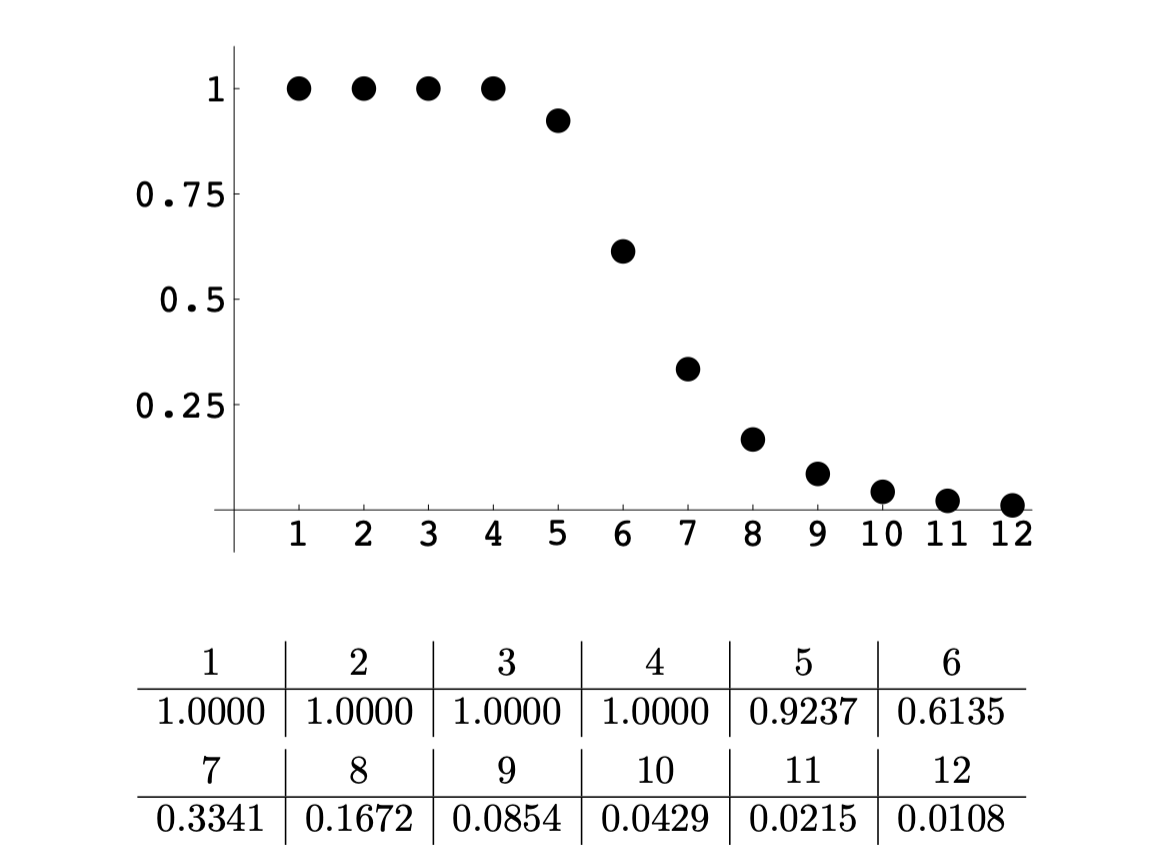
\includegraphics[scale=0.4]{convfig}

\caption{\protect\label{fig:seven-shuffle}$n=52,1\protect\leq k\protect\leq12$}

\end{figure}

\cite{Bayer_1992} also gave the asymptotic result: if $n$ cards
are riffle shuffled $k=\frac{3}{2}\log_{2}(n)+c$ times, then for
large $n$, 
\begin{equation}
\nm{P^{k}-U}=1-2\Phi\Bigl(\frac{-2^{-c}}{4\sqrt{3}}\Bigr)+O(n^{-1/4}),\label{eq:riffle-asymp}
\end{equation}
where $n$ is the normal CDF. Hence $\tmix^{(n)}=\frac{3}{2}\log_{2}(n)$.

\section*{The cutoff phenomenon}

The main results \eqref{eq:up-low-top} and \eqref{eq:riffle-asymp}
are very similar in nature, which is known as the cutoff phenomenon.
A bit informally, we call a sequence of Markov chains indexed by the
state space size $n$ has a \df{cutoff} at $k_{0}$ if $d\bigl(k_{0}+o(k_{0})\bigr)\approx0$
and $d\bigl(k_{0}-o(k_{0})\bigr)\approx1$. See figure \ref{fig:cutoff-plot}.
Asymptotically as $n\to\infty$ we should see the plot becoming a
step function at $k_{0}$. Of course $k_{0}$ is just $\tmix^{(n)}$.\footnote{We refer to chapter 18 of \cite{Levin_Peres_Wilmer_2017} for a more
general and precise definition of the cutoff phenomenon.} 
\begin{figure}[ht]
\centering
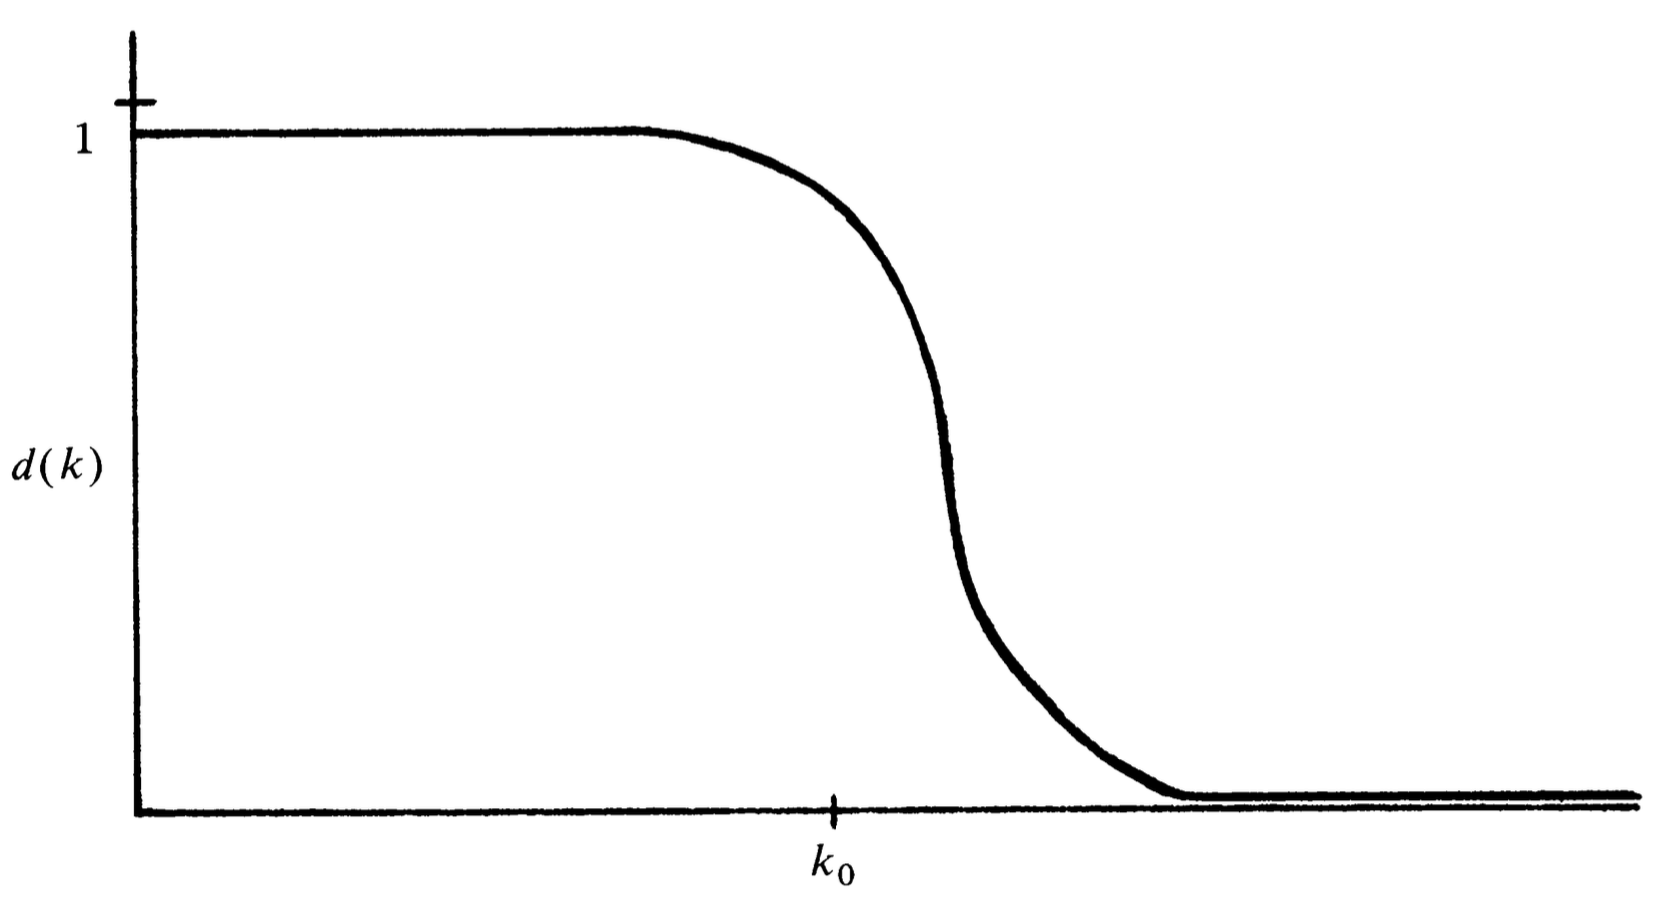
\includegraphics[scale=0.3]{cutoff}

\caption{\protect\label{fig:cutoff-plot}cutoff at $k_{0}$}

\end{figure}

It is clear that \eqref{eq:up-low-top} and \eqref{eq:riffle-asymp}
are examples of the cutoff phenomenon, and in fact most shuffle models
have this phenomenon. Note that even for a relatively small $n=52$,
the cutoff phenomenon in figure \ref{fig:seven-shuffle} is already
quite evident.

\newpage
\nocite{*}
\printbibliography

\let\thefootnote\relax\footnotetext{Our treatment mostly follows \cite{Levin_Peres_Wilmer_2017}, with inspirations from the other sources as well.}
\end{document}
